\documentclass[a4paper]{article}
\usepackage[margin=2cm]{geometry}
\usepackage{fontspec}

\usepackage[catalan]{babel}
\usepackage{amsmath}
\usepackage{amssymb}

\usepackage{csquotes}
\usepackage{graphicx}
\usepackage{float}

\setlength{\parindent}{0pt}
\setlength{\parskip}{1em}

\title{
	\textsc{Resum Termodinàmica} \\
	Tema 1
}

\author{Joan Marcè i Igual}

\begin{document}
\maketitle

\section{Definicions}

\begin{description}
	\item[Substància pura] És aquella que té una composició química homogènia i invariable. Pot existir en més d'una fase, però té la mateixa composició en totes les fases.
	\item[Postulat d'estat] El nombre de variables (intensives, molars o específiques) independents necessàries per caracteritzar l'estat d'un sistema de massa i composició constants és igual al nombre de treballs potencialment reversibles més un.
	\item[Variables intensives] Les variables intensives no depenen de la massa (P, T).
	\item[Variables específiques i molar] Les variables específiques o molars són extensives (V, H) i són la seva magnitud dividida per la massa o el nombre de mols i no depenen de la massa ($v = \frac{V}{m} \quad v = \frac{V}{n} \quad h = \frac{H}{m} \quad h = \frac{H}{n}$).
\end{description}

\section{Superfície PVT}

La superfície PVT és característica de cada element.

\begin{figure}[H]
	\centering
	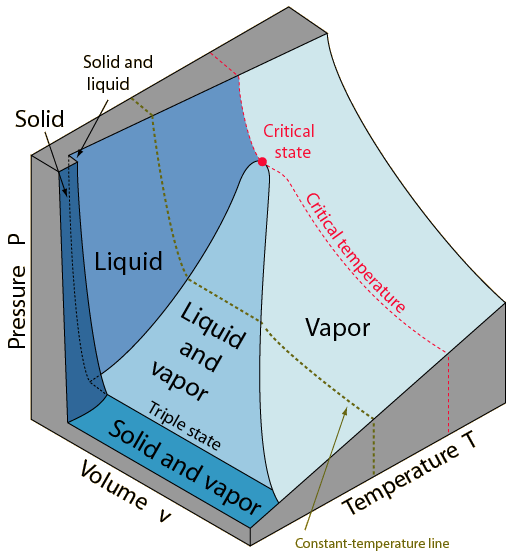
\includegraphics[width=0.5\linewidth]{superficie_PVT}
\end{figure}

\section{Mescla saturada líquid-vapor. Títol x}

El títol ($x$) és la proporció de massa de vapor respecte la massa total.

\begin{align*}
	\text{Títol: } &x = \frac{m_{vapor}}{m_{total}} = \frac{m_{v}}{m_v + m_l} \\
	\text{Humitat: } &1 - x = \frac{m_{líquid}}{m_{total}} = \frac{m_l}{m_v + m_l}
\end{align*}

\begin{figure}[H]
	\centering
	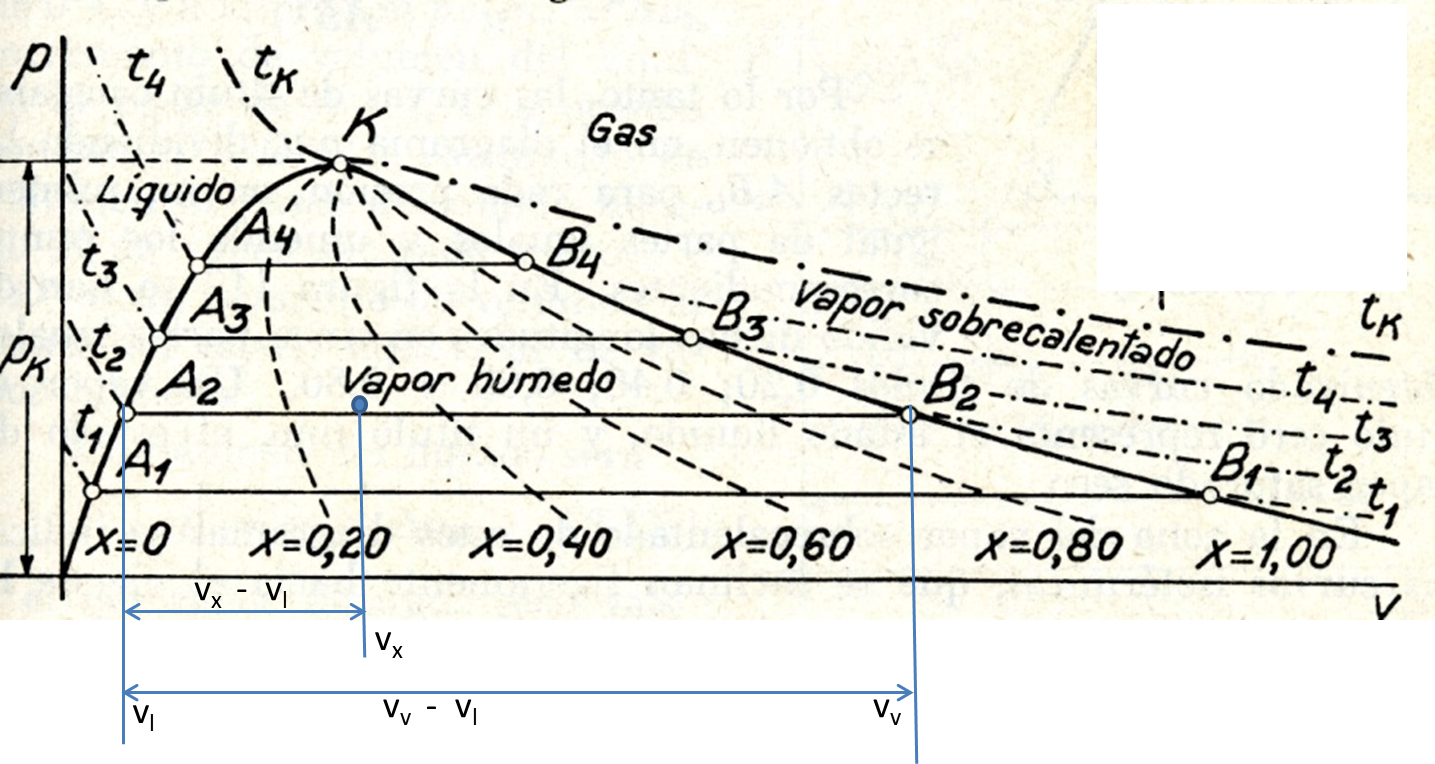
\includegraphics[width=\textwidth]{titol_vapor}
\end{figure}

Relacions entre propietats:
\begin{align*}
	V_v &= m_v V_v & V_l &= m_l v_l \\
	V &= V_v + V_l & m &= m_v + m_l
\end{align*}
\begin{align*}
	& v = \frac{V}{m} = \frac{V_v + V_l}{m_v + m_l} = \frac{m_v v_v + m_l v_l}{m_v + m_l}\\
	& v = x v_v + (1 - x) v_l \\
	& \boxed{x = \frac{v - v_l}{v_v - v_l}} \rightarrow \parbox{10em}{\small Igualtat per qualsevol propietat especifica}
\end{align*}

\section{Taules de saturació de l'aigua}
\begin{itemize}
	\item Entrada amb \textbf{una sola variable} (P o T).
	\begin{description}
		\item[l] Líquid saturat
		\item[v] Vapor saturat
	\end{description}
	\item Amb el \textbf{títol} i les dades de saturació es poden conèixer les propietats de la mescla.
	\item Si les dades no estan tabulades cal interpolar 
	$\rightarrow y = (x - x_0) \frac{y_1 - y_0}{x_1 - x_0} + y_0$
	\item Entalpia de vaporització $\Delta h_{lv} = h_v - h_l$
\end{itemize}

\section{Taules de vapor reescalfat/líquid comprimit de l'aigua}
\begin{itemize}
	\item Entrada amb \textbf{dues variables} (normalment P i T)
	\item Dades donades per isòbares.
	\item $P=ct \cap T > T^{sat} \implies$ vapor rescalfat
	\item $P=ct \cap T < T^{sat} \implies$ vapor subrefredat
	\item $P=ct \cap T = T^{sat} \implies$ estats saturats
	\item Per sobre del punt crític tenim gas
\end{itemize}

\section{Equacions empíriques i del virial}

\begin{equation*}
	\tag{Equació Van der Waals}
	P = \frac{R T}{v - b} - \frac{a}{v^2} \qquad 
	a = \frac{27 R^2 T_c^2}{64 P_c} \qquad
	b = \frac{R T_c}{8 P_c}
\end{equation*}
\begin{equation*}
	\tag{Equació Redling-Kwong}
	P = \frac{R T}{v - b} - \frac{a}{T^{\frac{1}{2}} v (v + b)} \qquad
	a = \frac{0,42748 R^2 T_c^{2,5}}{P_c} \qquad
	b = \frac{0,08664 R T_c}{P_c}
\end{equation*}
\begin{align*}
	\tag{Equacions del Virial}
	& z = 1 + \frac{B}{v} + \frac{C}{v^2} + \frac{D}{v^3} + ... \\
	& z = 1 + B'P + C'P^2 + D'P^3 + ...
\end{align*}

\section{Factor de compressibilitat Z}
És la desviació d'un gas real respecte el seu comportament de gas ideal. És un paràmetre adimensional que fa de relació entre propietats.

$$
Z = \frac{v_{real}}{v_{ideal}} = \frac{v_{real}}{\frac{R T}{P}} \implies
z = \frac{P v}{R T}
$$

\subsection{Principi dels estats corresponents}
\begin{itemize}
	\item Totes les substàncies a la mateixa $P_R$ i $T_R$ ocupen el mateix $v_R$. Així doncs $v_R = v_R(P_R, T_R)$.
	\item El factor de compressibilitat $Z$ és només funció de $P_R$ i $T_R$.
	\item Factor de compressibilitat generalitzat $Z = Z(P_R, T_R)$.
\end{itemize}
\begin{equation*}
	\tag{Variables reduïdes}
	P_R = \frac{P}{P_c} \qquad
	T_R = \frac{T}{T_c} \quad
	V_R = \frac{V}{V_c}
\end{equation*}

$$
v'_R = \frac{v}{\frac{R T_c}{P_c}}
$$

\begin{figure}[H]
	\centering
	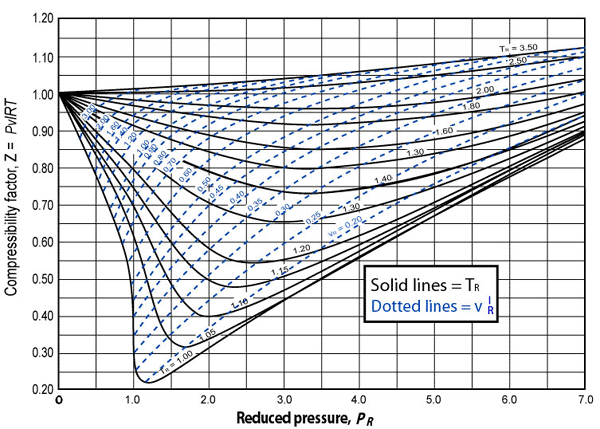
\includegraphics[width=\textwidth]{grafic_compressibilitat_z}
\end{figure}
\end{document}